\documentclass[oneside, 11pt]{article}

\usepackage[T1]{fontenc}
\usepackage[utf8]{inputenc}
\usepackage[english]{babel}

\usepackage{fouriernc}
\usepackage[detect-all, binary-units, separate-uncertainty=true,
            per-mode=symbol, retain-explicit-plus, retain-unity-mantissa=false]{siunitx}

\usepackage{setspace}
\setstretch{1.2}

\setlength{\parskip}{\smallskipamount}
\setlength{\parindent}{0pt}

\usepackage[headheight=14pt]{geometry}
\geometry{marginparwidth=0.5cm, verbose, a4paper, tmargin=3cm, bmargin=3cm,
          lmargin=2cm, rmargin=2cm}

\usepackage{float}

\usepackage[fleqn]{amsmath}
\numberwithin{equation}{section}
\numberwithin{figure}{section}

\usepackage{graphicx}
\graphicspath{{images/}{../../../images/}}

\usepackage{tikz}
\usetikzlibrary{shapes}
\usetikzlibrary{plotmarks}

\newcounter{Exercise}
\setcounter{Exercise}{1}
\usepackage{xcolor}
\definecolor{shadecolor}{gray}{0.9}
\usepackage{framed}
\usepackage{caption}

\usepackage{url}


\usepackage{fancyhdr}
\pagestyle{fancy}
\fancyhf{}
\rhead{\thepage}
\renewcommand{\footrulewidth}{0pt}
\renewcommand{\headrulewidth}{0pt}

\fancypagestyle{firststyle}
{
    \fancyhf{}
    \rhead{\thepage}
    \cfoot{
\includegraphics[height=30pt]{HiSPARClogo}}
    \rfoot{
\includegraphics[height=25pt]{CCbysa}}
    \lfoot{
\includegraphics[height=30pt]{NIKHEFlogo}}
    \renewcommand{\footskip}{50pt}
    \renewcommand{\footrulewidth}{0.1pt}
    \renewcommand{\headrulewidth}{0pt}
}

\newcommand{\figref}[1]{Figuur~\ref{#1}}

\newcommand{\hisparc}{\textsmaller{HiSPARC}\xspace}
\newcommand{\kascade}{\textsmaller{KASCADE}\xspace}
\newcommand{\sapphire}{\textsmaller{SAPPHiRE}\xspace}
\newcommand{\jsparc}{\textsmaller{jSparc}\xspace}
\newcommand{\hdf}{\textsmaller{HDF5}\xspace}
\newcommand{\aires}{\textsmaller{AIRES}\xspace}
\newcommand{\csv}{\textsmaller{CSV}\xspace}
\newcommand{\python}{\textsmaller{PYTHON}\xspace}
\newcommand{\corsika}{\textsmaller{CORSIKA}\xspace}
\newcommand{\labview}{\textsmaller{LabVIEW}\xspace}
\newcommand{\daq}{\textsmaller{DAQ}\xspace}
\newcommand{\adc}{\textsmaller{ADC}\xspace}
\newcommand{\hi}{\textsc{h i}\xspace}
\newcommand{\hii}{\textsc{h ii}\xspace}
\newcommand{\mip}{\textsmaller{MIP}\xspace}
\newcommand{\hisparcii}{\textsmaller{HiSPARC II}\xspace}
\newcommand{\hisparciii}{\textsmaller{HiSPARC III}\xspace}

\DeclareSIUnit{\electronvolt}{\ensuremath{\mathrm{e\!\!\:V}}}

\DeclareSIUnit{\unitsigma}{\ensuremath{\sigma}}
\DeclareSIUnit{\mip}{\textsmaller{MIP}}
\DeclareSIUnit{\adc}{\textsmaller{ADC}}

\DeclareSIUnit{\gauss}{G}
\DeclareSIUnit{\parsec}{pc}
\DeclareSIUnit{\year}{yr}



\begin{document}

\title{De Zon}
\author{N.G. Schultheiss}
\date{}

\maketitle
\thispagestyle{firststyle}

\section{Inleiding}

Deze module is direct vanaf de derde of vierde klas te volgen en wordt
vervolgd met de module ``De Broglie'' of de module ``Zonnewind''.
\begin{figure}[H]
\noindent \begin{centering}
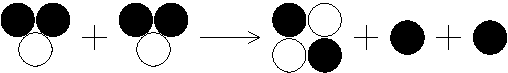
\includegraphics[scale=0.5]{fusie}
\par\end{centering}

\caption{Een schema voor kernfusie}
\end{figure}


In figuur 1.1 zien we een schematische voorstelling voor kernfusie. De
zwarte bolletjes stellen protonen voor en de witte bolletjes stellen
neutronen voor. Een deel van de kernreacties herverdelen de protonen en
neutronen over de kernen. Relatief kleine kernen zijn goed te tekenen.
Helaas zijn er ook veel grotere kernen. Van nature treedt kernfusie
globaal op van waterstof tot aan het element ijzer \footnote{Het kost
extra moeite om grotere atomen te maken omdat de protonen elkaar
afstoten. Grotere atomen hebben eerder de neiging om te splitsen als dan
om samen te smelten.}. Het element ijzer bevat altijd 26 protonen, het
atoomnummer \emph{Z} van ijzer is daarom 26. Verder bevat ijzer 54 tot
60 kerndeeltjes, het massagetal \emph{A} van ijzer ligt dus tussen 54 en
60. IJzer heeft dus $54-26=28$ tot $60-26=34$ neutronen. Het is dus niet
handig om een kernreactie met ijzer op de manier van figuur 1 te tekenen.

Scheikundig zijn dit allemaal ijzer-atomen. Toch heeft ieder ijzeratoom
eigenschappen, zoals radioactiviteit, die bij de massa van het atoom
horen. IJzer wordt daarom verdeeld in Fe-54, Fe-55, Fe-56, Fe-57,
Fe-58, Fe-59 en Fe-60 isotopen. Sommige isotopen zijn radioactief,
andere zijn niet radioactief of stabiel.

Het aantal protonen bepaalt welk scheikundig element het atoom is,
dit wordt ook wel het atoomnummer \emph{Z} genoemd. Het aantal kerndeeltjes
bepaalt het isotoop, dit wordt ook wel het massagetal \emph{A} genoemd.
Een isotoop is nu als volgt te noteren:
\[
_{Z}^{A}Symbool
\]


In figuur 1.1 zien we drie soorten isotopen. Isotopen met 3 kerndeeltjes
(2 protronen en 1 neutron), 4 kerndeeltjes (2 protronen en 2 neutronen)
en losse protonen. Atomen met 2 protonen maken deel uit van de He-familie
(helium). Atomen met 1 proton maken deel uit van de H-familie (waterstof).
Deze figuur is dus als volgt te noteren:

\[
2_{2}^{3}He^{2+}\rightarrow_{2}^{4}He^{2+}+2_{1}^{1}H^{+}
\]


Twee helium-3 isotopen botsen, er ontstaat een nieuw helium-4 isotoop
doordat een helium-3 isotoop een neutron overdraagt. De twee overgebleven
protonen vliegen uit elkaar en er ontstaan twee waterstof-1 isotopen.


\section{Zonne-energie}

De Zon is net als andere sterren een hemellichaam dat het grootste
deel van de uitgestraalde energie uit kernfusie haalt. De meeste energie
wordt op de zon vrijgemaakt door waterstofkernen (protonen) in een
aantal stappen om te zetten in Heliumkernen. 

Dit gaat op de volgende manier:
\begin{equation}
2_{1}^{1}H^{+}\rightarrow_{1}^{2}H^{+}+_{1}^{0}e^{+}+_{0}^{0}\nu
\end{equation}


\begin{equation}
_{1}^{2}H^{+}+_{1}^{1}H^{+}\rightarrow_{2}^{3}He^{2+}+_{0}^{0}\gamma
\end{equation}


\begin{equation}
\begin{array}{c}
2_{2}^{3}He^{2+}\rightarrow_{2}^{4}He^{2+}+2_{1}^{1}H^{+}\\
_{2}^{3}He^{2+}+_{1}^{1}H^{+}\rightarrow_{2}^{4}He^{2+}+_{1}^{0}e^{+}+_{0}^{0}\nu
\end{array}
\end{equation}
 

In de eerste vergelijking van 2.3 is niets bijzonders aan de hand,
de protonen en neutronen worden anders in de kernen gerangschikt.
Dit rangschikken van protonen en neutronen gebeurt ook in vergelijking
2.2. Omdat er maar 1 deeltje ontstaat, komt de energie echter vrij
in een flits, een $\gamma$-foton (gamma foton). Op fotonen komen
we nog terug.

Bij vergelijking 2.1 en de tweede vergelijking van 2.3 is er ook iets
aan de hand, hier wordt een proton omgezet in een neutron. Omdat de
lading voor en na de reactie hetzelfde te houden onstaat er een nieuw
deeltje, een positief electron of een positron. Het blijkt dat er
naast de lading nog een eigenschap van deeltjes behouden moet blijven,
de spin. Omdat protonen, neutronen en electronen een spin van $+\frac{1}{2}$
of $-\frac{1}{2}$ hebben, is er nog een extra deeltje met spin $+\frac{1}{2}$
of $-\frac{1}{2}$ nodig. Dit is een neutraal electron of neutrino
($\nu$).

Neutrino's vliegen overal bijna ongehinderd doorheen. Ze gaan bijvoorbeeld
bijna allemaal dwars door de Aarde. Heel af en toe botst er een neutrino
op deeltje en gebeurd er iets.

Positronen hebben veel meer moeite om ergens doorheen te vliegen.
De lading van de positronen zorgt dat ze veel eerder worden aangetrokken
door negatieve ladingen, zoals electronen. Als een electron en een
positron botsen, vindt de volgende reactie plaats:

\begin{equation}
_{1}^{0}e^{+}+_{-1}^{0}e^{-}\rightarrow2_{0}^{0}\gamma
\end{equation}


Beide deeltjes verdwijnen en er onstaan twee $\gamma$-fotonen. Als
een materie en een antimateriedeeltje precies recht op elkaar botsen,
verdwijnen ze. Omdat het electron en het positron beide verdwijnen,
kunnen we zeggen dat een positron een antimateriedeeltje van een electron
is. Als er maar één foton ontstaat kan dit zich nergens tegen afzetten.
Er moeten dus twee fotonen ontstaan die zich tegen elkaar afzetten,
zodat beide fotonen de lichtsnelheid kunnen krijgen.

Een $\gamma$-foton is eigenlijk een soort lichtflitsje met heel veel
energie. Het is geen materie en ook geen antimaterie, het foton hoort
bij de familie van de electromagnetische straling. Omdat electromagnetische
straling geen (rust-)massa heeft, moeten we een andere eigenschap
gebruiken om soorten electromagnetische straling te onderscheiden.
Iedere soort electromagnetische straling heeft een eigen golflengte.
Van een grote naar een kleine golflengte vinden we achtereenvolgens:
Radiogolven, Mobiele telefonie, Radar, Infrarode straling, Zichtbaar
licht (Rood, Oranje, Geel, Groen, Blauw, Violet), Ultraviolet, Röntgen
en Gamma-straling.


\paragraph*{Opdracht 1:}

\emph{Zoek de golflengten van Radiogolven, Mobiele telefonie, Radar,
Infrarode straling, Zichtbaar licht (Rood, Oranje, Geel, Groen, Blauw,
Violet), Ultraviolet, Röntgen en Gamma-straling op.}

Alle electromagnetische golven bewegen in vacuum met de lichtsnelheid
$c=299792458[\mathrm{m/s}]$, bij benadering is dit $300.000[\mathrm{km/s}]$.


\paragraph*{Opdracht 2:}

\emph{Bereken de frequentie van de verschillende soorten electromagnetische
golven.}

Het blijkt dat de frequentie recht evenredig is met de energie van
de fotonen.


\paragraph*{Opdracht 3:}

\emph{Beargumenteer waarom UV-stralen voor mensen wel gevaarlijk zijn
en zichtbaar licht niet. Waarom mag je niet teveel Röntgen foto's
maken?}


\paragraph*{Opdracht 4:}

\emph{Op
http://www.astro.ubc.ca/\textasciitilde{}scharein/a311/Sim/fusion/Fusion.html
kun je een simulatie van kernfusie zien. Bekijk deze en onderzoek
wat er gebeurd als het aantal protonen en / of de temperatuur wordt
verhoogd.}


\section{Zonnestralen}

De zon produceert zonnestralen. Zoals in hoofdstuk 2 te zien is, worden
$\gamma$-stralen door kernfusie geproduceerd. Gelukkig is dit maar
een klein deel van de zonnestraling. De meeste zonnestraling is te
zien als zichtbaar licht.

Men probeert op Aarde ook kernfusie-reactors te maken. Zoals uit opdracht
4 blijkt, is het echter niet eenvoudig omdat er voor een kernfusie
reactie een grote druk en een grote temperatuur nodig zijn. Beide
zijn in de Zon aanwezig. De zwaartekracht bij de Zon is groot, dit
komt omdat bijna alle massa van het zonnestelsel in de zon zit. De
druk in de Zon wordt dus ook erg groot. Alles is ooit in de zon gevallen,
de energie die bij dit vallen vrij kwam, werd omgezet in bewegingsenergie
van de atoomkernen. De temperatuur werd daardoor ook erg hoog. Door
de hoge druk en de hoge temperatuur start kernfusie. Als deze gestart
is, kan de zon deze kernenergie gebruiken om warm te blijven.


\paragraph*{Opdracht 5:}

\emph{Beredeneer waar de kernfusie in de zon plaats vindt.}

Het zichtbaar oppervlak van de zon, de fotosfeer heeft een temperatuur
die, als we in de zon af zouden dalen, van 4500K naar 6500K oploopt.
De zon is hier welliswaar gloeiend heet, de temperatuur is echter
veel te laag voor kernfusie. Het gloeien van het gas in de fotosfeer
zien wij als zonlicht. 


\paragraph*{Opdracht 6:}

\emph{Volgens Charles Darwin overleeft de meest passende soort door
natuurlijke selectie. Beredeneer met het model van Darwin hoe het
komt dat de zon hoofdzakelijk zichtbaar licht uitstraalt.}


\paragraph*{Opdracht 7:}

\emph{Beredeneer waarom de zon relatief weinig $\gamma$-straling
uitzendt.}


\section{Fotosfeer en Chromosfeer}

Zoals hiervoor te lezen is, is de fotosfeer het lichte deel dat we
normaal als de zon zien. Omdat de fotosfeer witheet is, geeft de zon
ook ``wit'' licht af. Dit is te vergelijken met een spijker die
je in een vlam houdt, eerst wordt deze roodgloeiend. Als de vlam heet
genoeg is, wordt de spijker na een tijdje witheet. In wit licht zitten
alle kleuren: rood, oranje, geel, groen, blauw, violet. Het licht
van de fotosfeer bevat dan ook alle kleuren.

Rond de fotosfeer is de chromosfeer. Het licht dat naar de aarde gaat
moet dus eerst door de chromosfeer. Deze is veel ijler dan de fotosfeer.
De fotosfeer is overigens al veel ijler dan de atmosfeer van de aarde.

\begin{figure}[h]
\centering
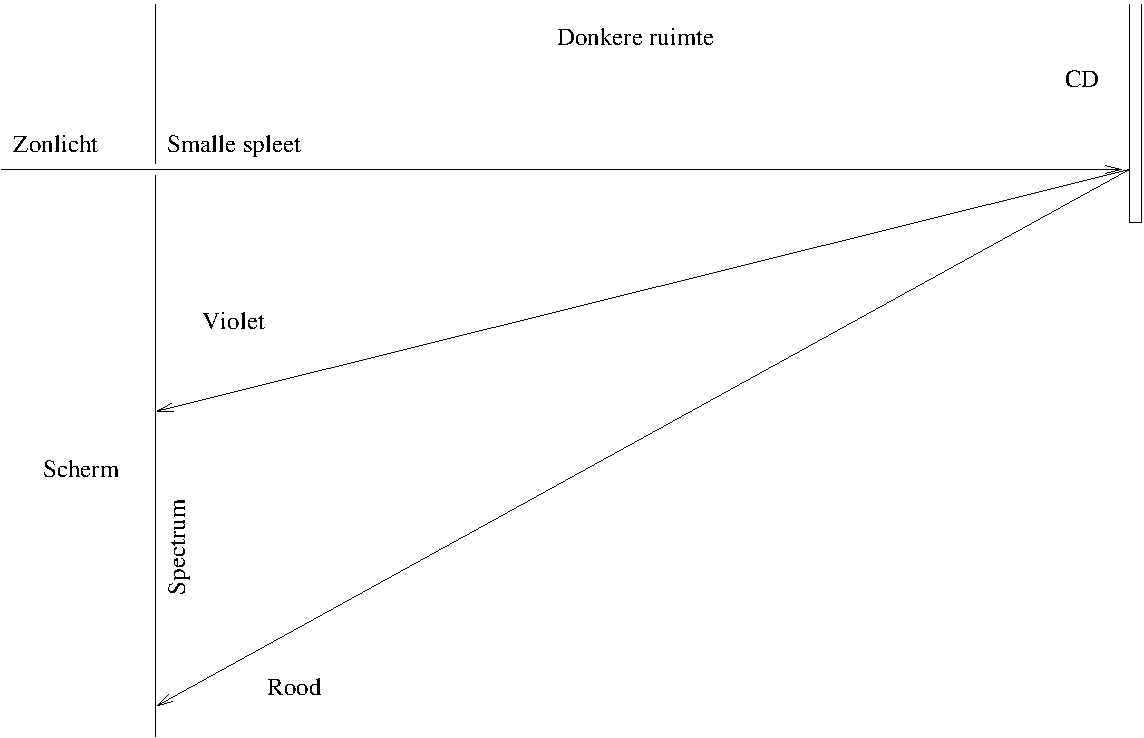
\includegraphics[scale=0.6]{zonlicht}

\caption{Een opstelling om het licht van de zon te bekijken}
\end{figure}


In chromosfeer wordt een deel van de kleuren van het licht geabsorbeerd.
Als je de kleuren van de fotosfeer van de zon met een prisma of CD
onderzoekt, krijg je een spectrum. Sommige kleuren zijn bijna niet
te zien, deze worden geabsorbeerd in de chromosfeer.


\paragraph*{Opdracht 8:}

\emph{Met wat knutselen kun je de opstelling in figuur 2 zelf maken.
Het licht valt valt op het gegroefde deel van de CD. Het is een hele
kunst om een scherp spectrum te maken. Het eerste wat opvalt is namelijk
dat zonlicht niet echt evenwijdig is. Als je de CD een meter van de
spleet in het scherm houdt, zie je dat het verlichte deel op de CD
breder is dan de spleet. Hiervoor is de corrigeren door een leesbril
met sterkte +1(dioptrieën) direct voor de CD te houden. Achter op
het scherm zie je met wat geluk een spectrum met zwarte lijnen.}

Het blijkt dat de chromosfeer zelf ook licht uitstraald. Dit is echter
veel minder dan het licht van de fotosfeer. Dit is te zien bij een
zonsverduistering. Nu kijken we als het ware in de zijkant van de
chromosfeer. Het licht dat eerst werd geabsorbeerd, is nu als geëmiteerd
(uitgezonden) licht te zien. De ``donkere'' strepen in het spectrum
van de fotosfeer zijn dus als ``gekleurde'' strepen in de chromosfeer
te zien.


\paragraph*{Opdracht 9:}

\emph{Met wat knutselen is een ``zonsverduistering'' misschien wel
met lenzen na te maken. Als we de zon groot genoeg afbeelden kunnen
we het licht van de fotosfeer tegenhouden en kunnen we misschien de
chromosfeer zien. In de praktijk is dit vrij ingewikkeld. Het ontwerpen
en onderzoeken / bouwen van een chromosfeer kijker is een goed onderwerp
voor een profielwerkstuk.}

\end{document}
